\chapter{git}

\section{git简介}

\tikz \draw (0pt,0pt) -- (20pt,6pt);

\tikz \draw[thick,rounded corners=8pt]
(0,0) -- (0,2) -- (1,3.25) -- (2,2) -- (2,0) -- (0,2) -- (2,2) -- (0,0) -- (2,0);

\begin{tikzpicture}
  \draw (-1.5,0) -- (1.5,0);
  \draw (0,-1.5) -- (0,1.5);
\end{tikzpicture}

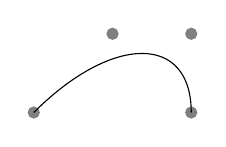
\begin{tikzpicture}
  \filldraw [gray] (0,0) circle (2pt)
  (1,1) circle (2pt)
  (2,1) circle (2pt)
  (2,0) circle (2pt);
  \draw (0,0) .. controls (1,1) and (2,1) .. (2,0);
\end{tikzpicture}

\tikz \foreach \x in {1,...,10}
\draw (\x,0) circle (0.4cm);

hello


\begin{tikzpicture}[
nonterminal/.style={
% The shape:
rectangle,
% The size:
minimum size=6mm,
% The border:
very thick,
draw=red!50!black!50, % 50% red and 50% black,
% and that mixed with 50% white
% The filling:
top color=white, % a shading that is white at the top...
bottom color=red!50!black!20, % and something else at the bottom
% Font
font=\itshape
}]
\node [nonterminal] {unsigned integer};
\end{tikzpicture}

hello

hello

\section{安装git}

\begin{verbatim}
sudo apt-get install git
sudo apt-get install git-core
\end{verbatim}

\section{创建版本库}

\begin{verbatim}
git config --global user.name "Laven Liu"
git config --global user.email "air.man.six@gmail.com"
\end{verbatim}

\section{本地仓库}

什么是版本库呢?版本库又名仓库,英文名repository,你可以简单理解成一个目录,这个目录里面的所有文件都可以被Git管理起来,每个文件的修改、删除,Git都能跟踪,以便任何时刻都可以追踪历史,或者在将来某个时刻可以“还原”。

所以,创建一个版本库非常简单,首先,选择一个合适的地方,创建一个空目录:

\begin{verbatim}
$ mkdir learngit
$ cd learngit
$ pwd
/Users/michael/learngit
\end{verbatim}

pwd命令用于显示当前目录。在我的Mac上,这个仓库位于/Users/michael/learngit。

如果你使用Windows系统,为了避免遇到各种莫名其妙的问题,请确保目录名(包括父目录)不包含中文。

第二步,通过git init命令把这个目录变成Git可以管理的仓库:

\begin{verbatim}
$ git init

\end{verbatim}

瞬间Git就把仓库建好了,而且告诉你是一个空的仓库(empty Git repository),细心的读者可以发现当前目录下多了一个.git的目录,这个目录是Git来跟踪管理版本库的,没事千万不要手动修改这个目录里面的文件,不然改乱了,就把Git仓库给破坏了。

首先这里再明确一下,所有的版本控制系统,其实只能跟踪文本文件的改动,比如TXT文件,网页,所有的程序代码等等,Git也不例外。版本控制系统可以告诉你每次的改动,比如在第5行加了一个单词“Linux”,在第8行删了一个单词“Windows”。而图片、视频这些二进制文件,虽然也能由版本控制系统管理,但没法跟踪文件的变化,只能把二进制文件每次改动串起来,也就是只知道图片从100KB改成了120KB,但到底改了啥,版本控制系统不知道,也没法知道。

不幸的是,Microsoft的Word格式是二进制格式,因此,版本控制系统是没法跟踪Word文件的改动的,前面我们举的例子只是为了演示,如果要真正使用版本控制系统,就要以纯文本方式编写文件。

因为文本是有编码的,比如中文有常用的GBK编码,日文有Shift\_JIS编码,如果没有历史遗留问题,强烈建议使用标准的UTF-8编码,所有语言使用同一种编码,既没有冲突,又被所有平台所支持。

言归正传,现在我们编写一个readme.txt文件,内容如下:

\begin{verbatim}
$ cat readme.txt
Git is a version control system.
Git is free software.
\end{verbatim}

一定要放到learngit目录下(子目录也行),因为这是一个Git仓库,放到其他地方Git再厉害也找不到这个文件。

和把大象放到冰箱需要3步相比,把一个文件放到Git仓库只需要两步。

第一步,用命令git add告诉Git,把文件添加到仓库:

\begin{verbatim}
$ git add readme.txt
\end{verbatim}

执行上面的命令,没有任何显示,这就对了,Unix的哲学是“没有消息就是好消息”,说明添加成功。

第二步,用命令git commit告诉Git,把文件提交到仓库:

\begin{verbatim}
$ git commit -m "wrote a readme file"
[master (root-commit) cb926e7] wrote a readme file
 1 file changed, 2 insertions(+)
 create mode 100644 readme.txt
\end{verbatim}

简单解释一下git commit命令,-m后面输入的是本次提交的说明,可以输入任意内容,当然最好是有意义的,这样你就能从历史记录里方便地找到改动记录。

嫌麻烦不想输入-m "xxx"行不行?确实有办法可以这么干,但是强烈不建议你这么干,因为输入说明对自己对别人阅读都很重要。实在不想输入说明的童鞋请自行Google,我不告诉你这个参数。

git commit命令执行成功后会告诉你,1个文件被改动(我们新添加的readme.txt文件),插入了两行内容(readme.txt有两行内容)。

为什么Git添加文件需要add,commit一共两步呢?因为commit可以一次提交很多文件,所以你可以多次add不同的文件,比如:

\begin{verbatim}
$ git add file1.txt
$ git add file2.txt
$ git add file3.txt
$ git commit -m "add 3 files."
\end{verbatim}

\subsection{版本回退}

\subsection{工作区和暂存区}

\subsection{管理修改}

\subsection{撤销修改}

\subsection{删除文件}

\section{远程仓库}

\subsection{添加远程库}

\subsection{克隆远程库}

\section{分支管理}

\subsection{创建与合并分支}

\subsection{解决冲突}

\subsection{分支管理策略}

\subsection{Bug分支}

\subsection{Feature分支}

\subsection{多人协作}

\section{标签管理}

\subsection{创建标签}

\subsection{操作标签}

\section{使用GitHub}

\section{自定义Git}

\subsection{忽略特殊文件}

\subsection{配置别名}

\subsection{搭建Git服务器}

